\chapter{Conclusion}
\label{chap: Chapter 8}

Based on the discussion in the previous chapter, it is clear that using the various natural language processing and text mining techniques outlined in Chapter \ref{chap: Chapter 6} would indeed be possible. It was apparent that adjusting the parameters of the prototype also played a major role in the quality of the topics. Later, such topics directly influenced the recommendation list.

This chapter provides a summary of the study to conclude the findings of the study. The next section will discuss how the research objectives were reached. After that section, suggestions will be made for future research.

\section{Revisiting the research objectives}

This section facilitates a discussion on how the research objectives were met. As mentioned in Chapter \ref{chap: Chapter 1}, the primary research objective was to \textbf{\textit{Develop a model to recommend related research papers.}}

Achieving the primary objective depended on meeting the secondary objectives listed in Chapter \ref{chap: Chapter 1}.

\textbf{SO 1}: \textit{To identify recommender systems techniques and how they are used.}

This secondary objective was met by surveying the literature about recommender systems. As the goal of this secondary objective was to map and understand which techniques are used in recommender systems and how researchers utilise it, I looked at the various approaches that not only fit the use case of the study but also at which are relevant. 

It was decided that the content-based filtering approach would the best to use since no assumptions are made about user activity. In addition to this, CBF does not care about user ratings; it looks at the content of the documents. It was critical to look for approaches that do not rely on user activity and user ratings. Chapter \ref{chap: Chapter 2} was dedicated to introducing the concepts of how modern information systems (Recommender Systems) work and how they have evolved from the past to recent years. A continuation of the introduction to the fields was found in Chapter \ref{chap: Chapter 3}.

\textbf{SO 2}: \textit{To identify machine learning techniques that assist with the recommender task.}

This secondary objective was met by surveying several machine learning techniques. The goal of this objective was to identify and understand better what machine learning techniques there are, and how they tie into recommender type systems. 

Machine learning in Section \ref{ssec:MLoverview}, natural language processing in Section \ref{secc:LDAover}, and topic modeling in Section \ref{ssec:tmodel} paved the way to understand the technology that would be used in this study.

The selection of the topic model algorithm that would be most suitable came from literature. More specifically, in Section \ref{ssec:tmodel} it was discussed that latent dirichlet allocation (LDA) was a very popular choice for building such topic models. Furthermore, Section \ref{ssec:LDAA} explains how LDA works, by computing hidden topic structures from documents.

The main research objective was met by consolidating \textbf{SO 1} and \textbf{SO 2} to form a conceptual model. The model was refined by developing a prototype. 

To develop such a model, some guidance was needed. The researcher used the data analytics lifecycle process to harness work done by secondary objectives one and two. Further refinement was needed on the model to display research rigour.

The development of the model was documented in Chapter \ref{chap: Chapter 5}, accompanied by the development of the prototype in Chapter \ref{chap: Chapter 6}. A prototype was developed to refine, ensure the amendments to be done, and showed whether the model is applicable and feasible. The model demonstrated applicability since it required domain-specific data for training and this was done using Information Security South Africa conference data. In addition, the model also demonstrated feasibility with its ease of using recommender system and machine learning techniques.

In the next section, a reflection on the model will be discussed.

\section{Reflection on the Model}

\begin{figure}[htbp]
\centering
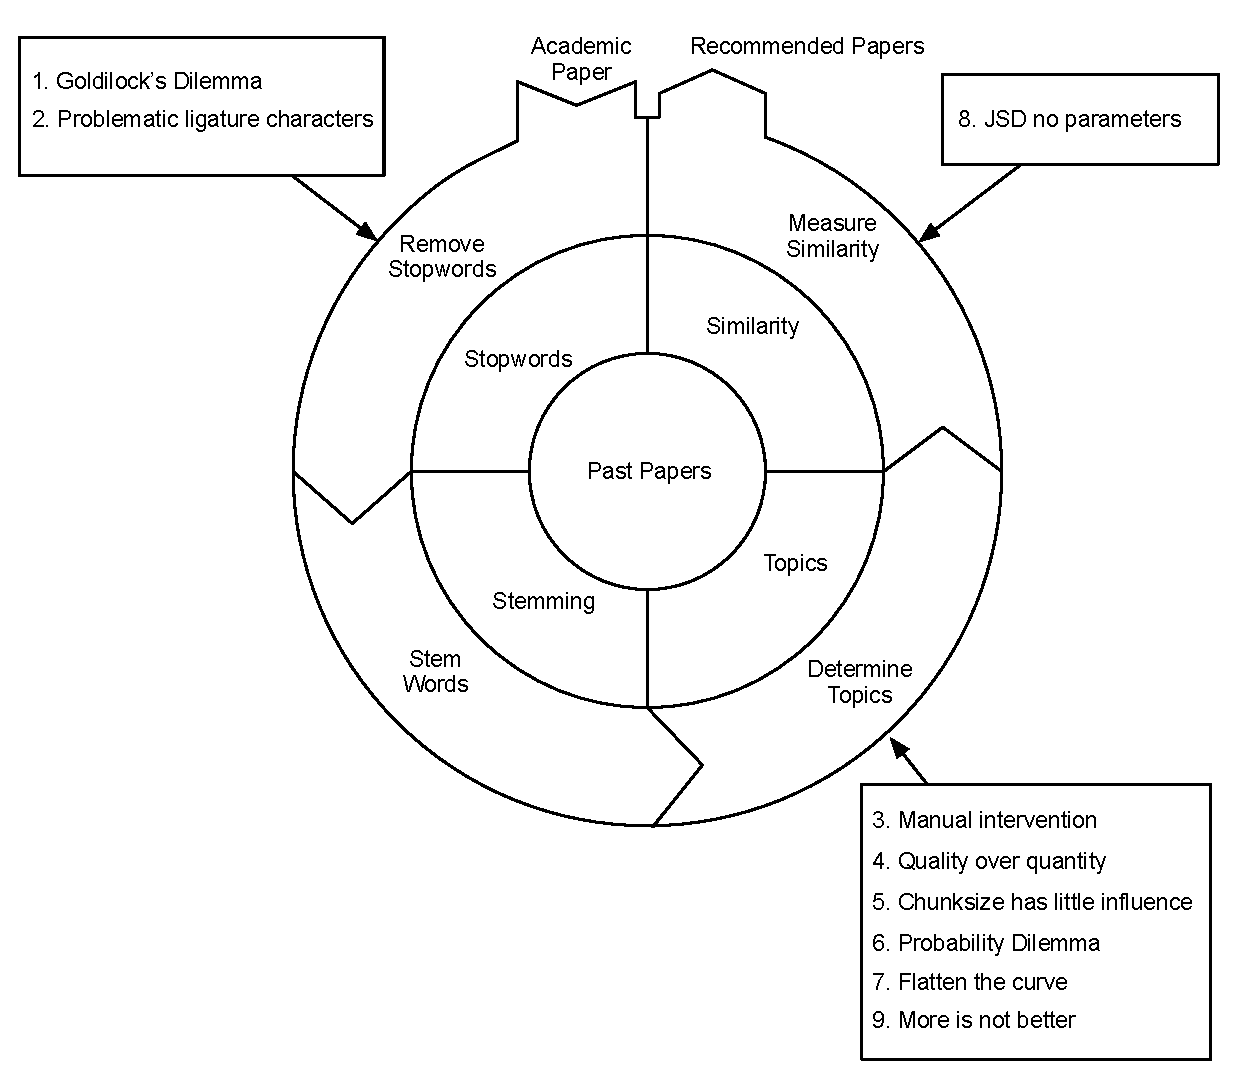
\includegraphics[width=15cm]{./figures/Lesson77.eps}
\caption{Mapping lessons learned to the model}
\label{fig:processing1}
\end{figure}

This section reflects on the model and the accompanying prototype. The model was developed to identify related research papers. The model specified the process that needs to be followed and the prototype showed that it is indeed feasible to implement. The prototype showed that it worked within the specific domain of information security papers, since we used Information Security South Africa conference papers from 2006–2016 as data. Addressing the main objective using the model and prototype, it was shown that it can be done, theoretically and practically.

The prototype served a dual purpose. The first was to learn technologies and to gain first-hand experience related to recommender systems. The second was to demonstrate its applicability by using various technologies and feasibility by using a information security specific domain. 

The majority of the lessons learned exists in the topics quadrant of the model, as depicted in Figure \ref{fig:processing1}. It was found that removing the stopwords and stemming the data meant that it was streamlined and the body of knowledge was well defined. Removing stopwords and stemming present two lessons to draw the attention of future researchers to the subtleties in the area. For testing similarity measures, only Jensen-Shannon Divergence was tested. Jensen-Shannon Divergence does not use parameters, and therefore had an big influence on the preceding steps.

This opens up opportunities for future research to be undertaken using different similarity measure technologies, which do contain parameters. 

To get back to the majority of the lessons about determining the topics. Lessons four, seven and nine show us that if we can define the domain better, the model will perform better. A trade-off thus exists between accuracy and generality. In the prototype, the domain was limited to information security papers by using research papers from the Information Security South Africa conference. 

Moving on to lesson three, manual intervention. It was found that evaluation techniques for machine learning algorithms are well defined and streamlined. However, human validation is needed, since bad topics still make it into the system, thus challenging future researchers to look for methods and techniques that eliminate such human intervention altogether.

\section{Research Limitations}

This study has some limitations that must be recognised. The first limitation is that of the sample size. At the time of data collection, the Information Security South Africa conference only had 254 research papers to use in the dataset. Of those 254 research papers, certain topics are only discussed in a limited number. If the topics are scarce during training, the recommendation task will be very difficult to complete. The goal was to train and test the prototype using one specific library of one conference.

The second limitation is that only one topic modeling technique (latent dirichlet allocation) was used. There were several reasons for this, one of which is that recent research suggests that when using content-based approaches, latent dirichlet allocation would be preferred. Considering time constraints, since this is a Master’s study, we felt it right to go ahead with the one topic modeling technique.

The third limitation is that this study only uses Jensen-Shannon Divergence to calculate the similarity between the two data spaces (test set and training set). Similar to the second limitation, time did not allow us to venture deeper into different similarity measures.
The fourth limitation includes not having a human factor to evaluate each phase individually. The phases which are referred to are the outputs of the topic modeling technique and also the end result of the similarity measurement.

Lastly, the fifth limitation is that this study did not compare how different recommender systems performed (optimisation and recommendations). This research study focused on documenting the process of using one recommender system and discussing the observations.

\section{Suggestions for further research}

This section is dedicated to outlining further research to be done on the limitations which were raised in the previous section. Future research could possibly be conducted using a conference that has more research papers at their disposal. It will provide more data to be clustered and will ultimately, better the similarity measures. This relates to the first limitation.

Reflecting on the second limitation, the study could include multiple topics modelling algorithms and compare the outputs. Examples of such algorithms are: non negative matrix factorisation (NMF) \cite{Purpura2018}, latent semantic analysis (LSA) \cite{Qomariyah2019}, parallel latent dirichlet allocation (PLDA) \cite{Mukherjee2019} and Pachinko allocation model (PAM) \cite{Koltcov2021}.

Similarly, the third limitation, using different similarity measures could lead to different recommendations. Furthermore, mixing different topic models with similarity measures could yield better results.

The fourth limitation, which includes human intervention to evaluate each phase, could speed up the model implementation, since one would be getting feedback every step of the way. Suggestions for further research can include looking for methods and techniques that eliminate manual intervention.

Reflecting on the fifth limitation, this study did not compare the performance and recommendations of different recommender systems. This limitation can be addressed in future research by considering alternative recommender systems. Examples of such recommender systems are: a hybrid model \cite{sharma2016evolution} and model-based collaborative filtering \cite{naak2009multi}. Future research could possibly be conducted using data sets which includes user-item pairing data.

\section{Epilogue}

This study identified that it is time consuming for researchers to look for related research papers. This problem was addressed by developing a model to recommend related research papers. 
Throughout the development of the model and prototype, it was evident that machine learning bridges the gap of spotting latent themes. However, Chapter \ref{chap: Chapter 7}, the lessons learned, shows that when other researchers endeavour to explore similar topics, a great learning curve awaits. The researcher hopes that this study will motivate other researchers to advance the research angle of the traditional topic of natural language processing and machine learning. 